\section{Method}

\begin{figure}
	\centering
	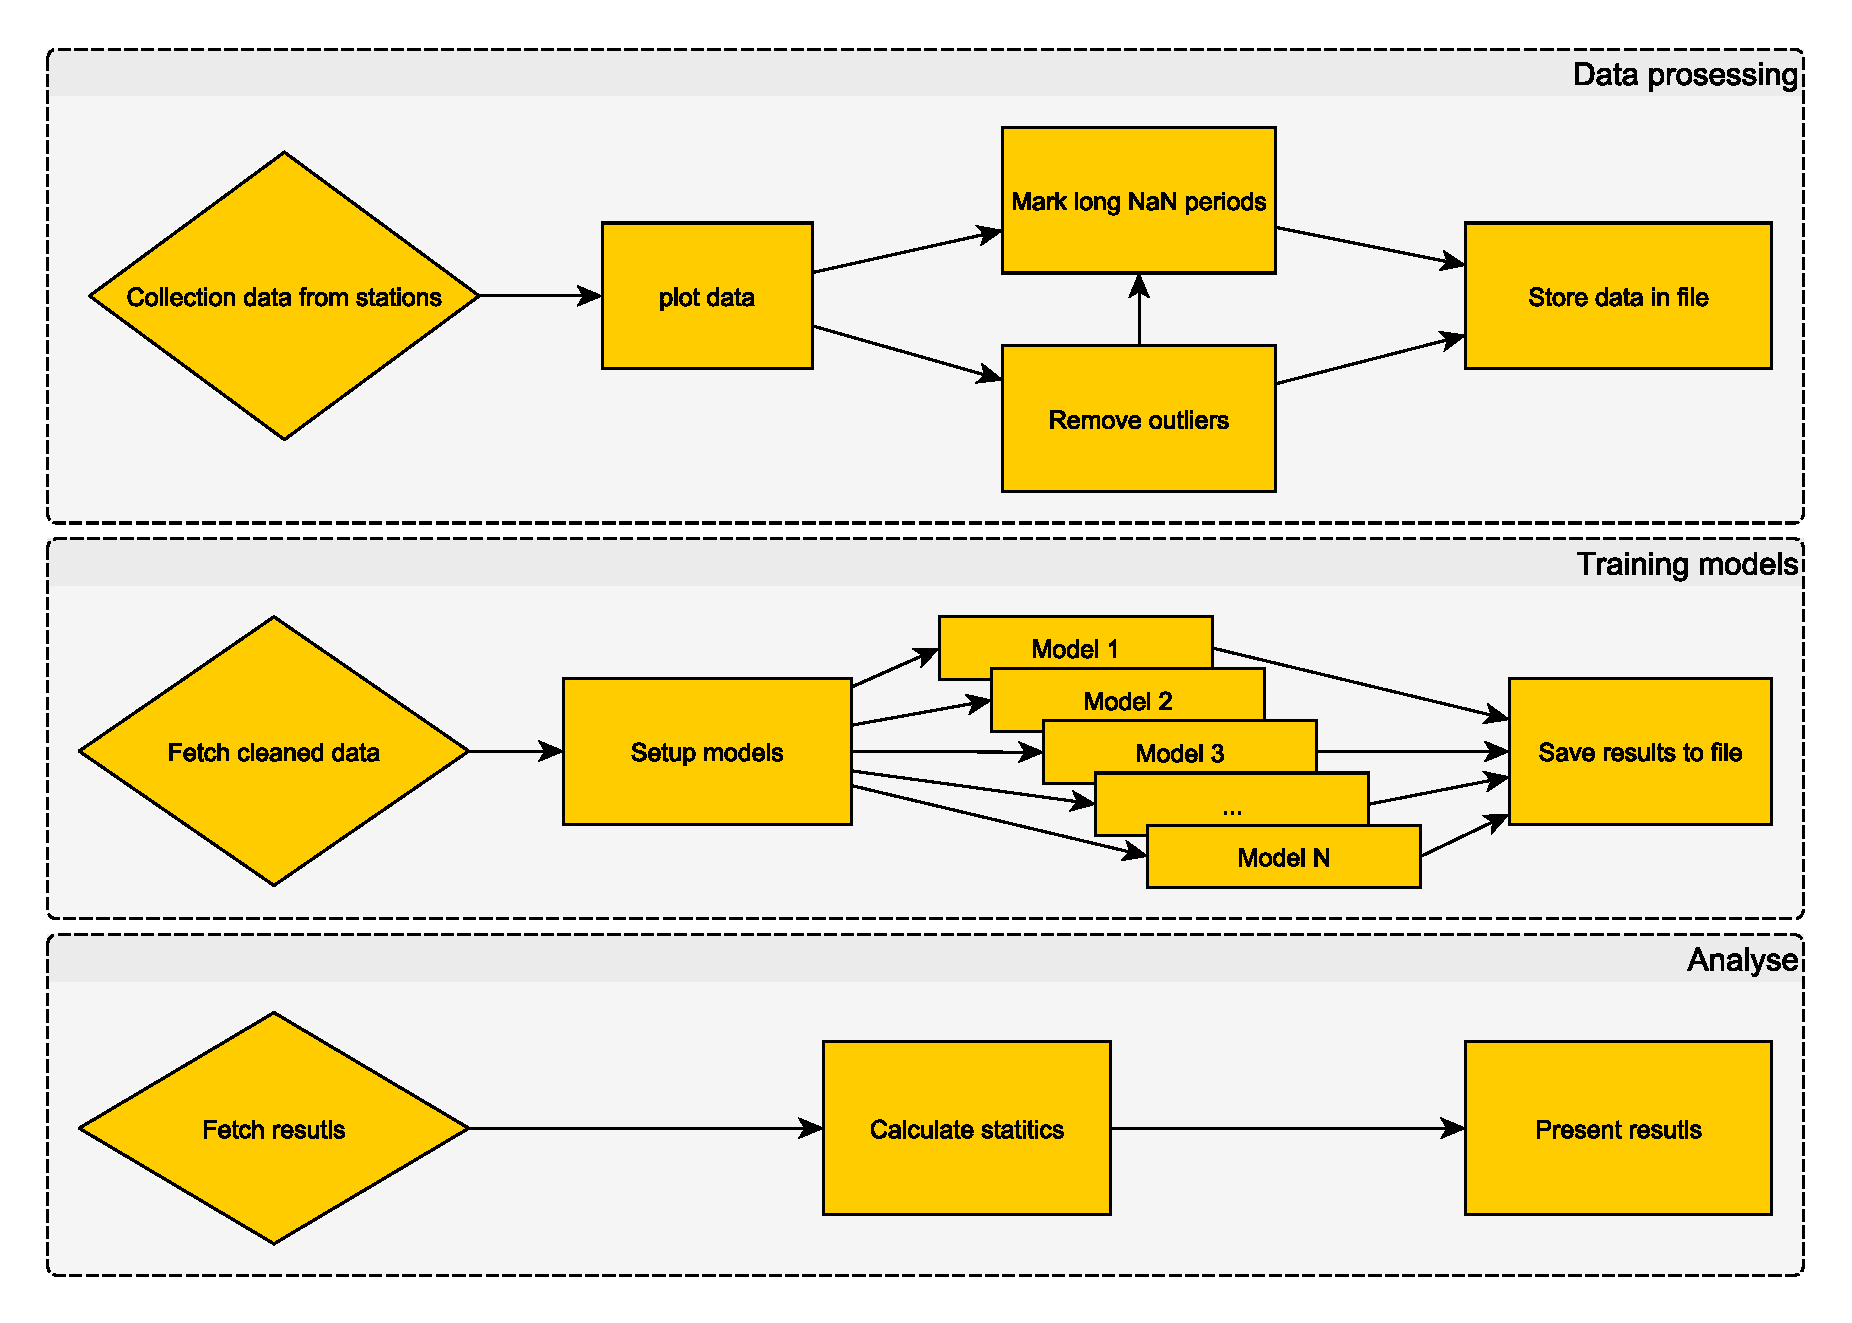
\includegraphics[width=0.7\linewidth]{figures/progress_diagram}
	\caption[Diagram sketching three procedures used in this study.]{A surface level diagram of the methodology.}
	\label{fig:progressdiagram}
\end{figure}\todo{Complete diagram}

\subsection{Source of data}

For this comparative study the following data sources will be used

\begin{enumerate*}
	\item \acrfull{ac:nibio}
	\item \acrfull{ac:kilden}
	\item \acrfull{ac:met}
\end{enumerate*}

\subsection{Dataset}

The dataset is chosen from four regions in Norway; Innlandet, Vestfold, Trøndelag, and Østfold. From each region are four stations picked:
\begin{table}[h]
	\begin{adjustwidth}{-1in}{-1in}
		\centering
		\begin{tabular}{llrlrrr}
			\hline Region&Name&ID&Drain type&MET name& Latitude&Longdetude\\\hline
			Innlandet&Apelsvoll&11& Selvdrenert&SN11500&60,70024&10,86952\\
			Innlandet& Fåvang&17& Selvdrenert&SN13150&61,45822&10,18720\\
			Innlandet& Ilseng&26& Selvdrenert&SN12180&60,80264&11,20298\\
			Innlandet& Kise&27& Vannmettet&SN12550&60,77324&10,80569\\
			Trøndelag& Kvithamar&57& Vannmettet&SN69150&63,48795&10,87994\\
			Trøndelag& Frosta&15& Selvdrenert&SN69655&63,56502&10,69298\\
			Trøndelag& Mære&34& Selvdrenert&SN71320&63,94244&11,42527\\
			Trøndelag& Rissa&39& Vannmettet&SN71320&63,58569&9,97007\\
			Vestfold& Lier&30& Vannmettet&SN19940&59,79084&10,25962\\
			Vestfold& Sande&42& Vannmettet&SN26990&59,61620&10,22339\\
			Vestfold& Tjølling&50& Selvdrenert&SN27780&59,04641&10,12513\\
			Vestfold& Ramnes&38& Vannmettet&SN27315&59,38081&10,23970\\
			Østfold& Rakkestad&37& Vannmettet&SN3290&59,38824&11,39042\\
			Østfold& Rygge&41& Selvdrenert&SN17380&59,39805&10,75427\\
			Østfold& Tomb&52& Vannmettet&SN17050&59,31893&10,81449\\
			Østfold& Øsaker&118& Vannmettet&SN3370&59,31936&11,04221\\\hline
		\end{tabular}
	\end{adjustwidth}
	\caption[Soil information for each station/w location and MET-ID]{Station information from stations used in this study. The MET names was found by looking at the coordinates of the station and finding the closest MET station coordinates.}
\end{table}

All stations are sampled from the date\footnote{Format month-day} 03-01 to 10-31 from 2016 to 2020. The features mean hourly soil temperature at 10cm (TJM10), mean hourly soil temperature at 20cm (TJM20), and mean hourly air temperature at 2m (TM) are sampled from the LMT database.

\subsubsection{Selection process}

An array of stations was provided by LMT based on their possession of the necessary data. All stations were reviewed, checked for missing data, and those with excessive gaps were removed from the list or replace with another station. After compiling a list of stations, each one was re-examined to identify outliers present in the data and eliminate them accordingly. If certain stations had an excessive number of missing values after the outlier check, nearby stations were sought, and the affected station was replaced and the outlier check was re-done. Table \ref{fig:plot-17} is showing station 17 (Apelsvoll, Innlandet) before treatment, and table \ref{fig:plot-17-treated} shows the same station cleaned and ready for being used as training/testing data.

\begin{figure}
		\centering
		\begin{adjustwidth}{-1in}{-1in}
			\includegraphics[height=0.9\textheight, width=\textwidth, angle=90]{"../../results/plots/Plot_test_naive_nan_k17_fTJM20.pdf"}
		\end{adjustwidth}
		\caption[Visual representation of station 17]{Visual representation of missing values at station 17 from 2014 to 2022 at the parameter "TJM20". The left numbers indicated how many hours that are missing and how many of them are shorter than or longer than 5 hours. The yellow markings indicate possible outliers based on the given year, all markings was checked if they were actual outliers. The red colouring indicate missing values in the data (represented in the data with code "NULL").}
		\label{fig:plot-17}
\end{figure}
\begin{figure}
		\centering
		\begin{adjustwidth}{-1in}{-1in}
			\includegraphics[height=0.9\textheight, width=\textwidth, angle=90]{"../../results/plots/Plot_test_naive_nan_treated_k17_fTJM20.pdf"}
		\end{adjustwidth}
		\caption[Visual representation of station 17 treated]{Visual representation of missing values at station 17 from 2014 to 2022 at the parameter "TJM20" after treating for outliers. The left numbers indicated how many hours that are missing and how many of them are shorter than or longer than 5 hours, however for this visualisation they indicate the untreated version of the data. The yellow markings indicate possible outliers based on the given year, all markings was checked if they were actual outliers. The red colouring indicate missing values in the data (represented in the data with code "NULL"). The years 2014 and 2015 was removed from the dataset but not coloured in due to technical limitations of reusable code, and furthermore half of 2016 was removed due to suspicion of misreading from sensor at this station.}
		\label{fig:plot-17-treated}
\end{figure}

The data plots (see figure \ref{fig:plot-17} and \ref{fig:plot-17-treated} as example) shows all the raw data plotted as a blue line from 03-01 to 10-31. The yellow markings is placed there by computer algorithmns (see section \ref{sec:method:outlier} for in-depth explanation of the outlier detection methods) as potential outliers in the data. These markings have been looked over and verified weather or not they are genuine outliers or not. Further more the red lines are indicators of missing values, the number of missing values longer or shorter than 5 hours\footnote{The threshold for rain is 3 hours due to the high variance.} are noted on the side bare with the total number of missing values regardless of length. The bottom bar are all the years laid on top of each other to highlight any years or periods that deviates for a particulate year compared to all the other years. There will be two versions of these plots, one for the untreated data and one for the treated data to show the difference the interpolation does to the data (see seciotn \ref{sec:method:interpolation} for further details.).

\subsubsection{Collection of data}

\begin{table}
	\begin{tabular}{lcc}
		Name       &                    version                    &                       description                        \\ \hline
		Powershell &                    7.3.11                     &            Windows native scripting language             \\
		Curl       & 8.4.0 (windows) libcurl/8.4.0 Schannel WinIDN & Commandline tool to communicate with servers using http. \\
		python     &                    3.9.11                     &                popular Scripting language
	\end{tabular}
	\caption[software version description]{The description the software used in this study}
	\label{tab:software}
\end{table}

In the tabel \ref{tab:software} are the softwares used in this study and in the collection and treatment of the data. The program used in the collection of meteorological messurements is Powershell in combination with Curl. Using hyperlinks gathered from inspecting \acrshort{ac:kilden}'s web page using the browser (Microsoft edge) built-in inspector tool to get the relevant links to send data requests. The presise URL's can be reviewed on GitHub in the studies GitHub repository\footnote{Link: https://github.com/ConAltDelete/MT24CS}. For a more surfac level description on what was requested of the servers see table \ref{tab:station_request}.

\begin{table}
	\centering
	\begin{tabular}{r|p{5cm}|}
		FROST & Description\\ \hline
		Station ID & Sendt a request to LMT for station information using their remote API.\\
		 \hline LMT & Description\\ \hline
		Meteorological data & Requested soil temperature from 10cm depth, and 20cm depth and air temperature (2m), from 2014-03-01 to 2022-10-31.
	\end{tabular}
	\caption[Request to servers about stations]{Description of what was requested from each server (\acrshort{ac:met}, \acrshort{ac:nibio}).}
	\label{tab:station_request}
\end{table}

\subsubsection{Storage of data}
The storage of the data is done through two data structures; \gls{gl:hashmap} and \gls{gl:dataframe} from the package pandas. The transformation of data is done with a customized data-type called "DataFileHandler" which is converted to a module for convenience. The keys for the hashmap is chosen by the naming of the data files and the pattern given to the class. To escalate the loading of the data it will also be exported to a binary file for faster retrieval. 

\paragraph[Data structure]{Technical overview of custom data structure}
The data structure used to store the data from the different stations is called "DataFileHandler" and stores the data in a nested dictionary which can be inpreted as the data structure "tree". The main features of "DataFileHandler" is 
\begin{enumerate}
	\item Simple syntax for partitioning the data
	\item Grouping the data after loading
	\item Transforming all the data with the same function
	\item loading and unloading of a large collection of data
\end{enumerate}

\subsection{Data cleaning and treatment}

To use the data in this study it must be cleaned and treated for training. Though the data has been examined by the supplier, however it still had outliers that needed to be treated before modelling. For this reason several steps and methods is utilized in the prepossessing steps. The selection process for finding these station can be compiled into these steps

\begin{enumerate}
	\item Recommendation from Norwegian Institute of Bio-economy Research
	\item \label{list:na_anal}Compute the missing values in the data
	\item Missing values analyse 
	\item Searching LMT database for alternative station candidates if current data is insufficient
	\item If some station was replaced the repeat step \ref{list:na_anal}
\end{enumerate}

\subsubsection{Outlier detection and removal}\label{sec:method:outlier}\todo{Revise so it reflects what you actually do}

Though the data fetched from \acrshort{ac:nibio} is treated and controlled the external data from \acrshort{ac:met} might not be, and this research project incorporated raw, untreated data from \acrshort{ac:nibio} to fill inn missing values.

The method to quickly find obvious outliers was to look at the following condition
\begin{equation}
	|z(|\Delta T|)| = \left|\frac{|\Delta T|-E(|\Delta T|)}{Var(|\Delta T|)}\right|> 4^\circ C
\end{equation}\todo{Make more clear}

Where the $E()$ is the expected value, and $Var()$ is the variance. This condition looks at the absolute difference between consecutive measurements and calculates the z-score for each observation. It is expected that the change in temperature can't be too rapid. Further methods used to highlight potential outliers is 

\begin{figure}[h]
	\centering
	\definecolor{zzttqq}{rgb}{0.6,0.2,0.}
	\definecolor{REDDD}{rgb}{0.8,0.5,0.2}
	\definecolor{ududff}{rgb}{0.30196078431372547,0.30196078431372547,1.}
	\begin{tikzpicture}[line cap=round,line join=round,>=triangle 45,x=1.0cm,y=1.0cm]
		\begin{axis}[
			x=1.0cm,y=1.0cm,
			axis lines=middle,
			ymajorgrids=true,
			xmajorgrids=true,
			xmin=-0.5,
			xmax=3.5,
			ymin=-0.5,
			ymax=2.5,
			xtick={-0.0,1.0,...,3.0},
			ytick={-0.0,1.0,...,2.0},]
			\clip(-0.5,-0.5) rectangle (3.5,2.5);
			\draw [line width=2.pt,dash pattern=on 1pt off 1pt] (1.04,1.02)-- (3.04,0.02);
			\draw [line width=2.pt] (1.04,1.02)-- (2.04,2.02);
			\draw [line width=2.pt] (2.04,2.02)-- (3.04,0.02);
			\begin{scriptsize}
				\draw [fill=ududff] (1.04,1.02) circle (2.5pt);
				\draw[color=ududff] (1.18,1.39) node {$A$};
				\draw [fill=ududff] (3.04,0.02) circle (1.5pt);
				\draw[color=ududff] (3.18,0.31) node {$B$};
				\draw [fill=ududff] (2.04,2.02) circle (1.5pt);
				\draw[color=ududff] (2.18,2.31) node {$C$};
				\draw [fill=zzttqq] (2.,0.54) circle (2.5pt);
				\draw [color=REDDD,dashed] (2.,0.54) circle (0.5);
				\draw[color=zzttqq] (2.14,0.91) node {$C^*$};
			\end{scriptsize}
		\end{axis}
	\end{tikzpicture}
	\caption[Simple Interpolation outlier detection]{An simple outlier detection method utilizing a simple line to estimate where the expected point ($C^*$,red dotted circle) is supposed to be. If observed point C falls outside the tolerance level (green circle) then it is marked as an outlier.}
\end{figure}

\subsubsection{Missing value imputation}\label{sec:method:interpolation}

The data has missing values, in particular during early Autumn when there were sub-zero temperatures meaning any rain measurements done during this period would have unpredictable fluctuations since at negative temperatures water can freeze, get clogged up with residual bio-material from the surrounding area \todo{Rewrite this part to reflect what is going on}. When interpolating values the method chosen is a linear interpolation with a maximum period of 5 consecutive hours for soil temperatures, and 3 consecutive hours for air temperatures. The reasoning for this is that the soil temperatures are more reliable makeing it safer to interpolate without loosing too much information, while air temperatures has a higher variance making it more difficult to interpolate without cutting values.

\subsubsection{Summary of data}

After going to the prosedure the current form of the station are

\begin{table}
	\begin{adjustwidth}{-1in}{-0.8in}
	\begin{tabular}{rllll}
\hline
      & 38   & 34   & 27   & 42   \\
\hline
 2014 & \begin{tabular}{ll}
\hline
 $\mu$:11.71  & max:31.8 \\
 $\sigma$:6.4 & min:-4.0 \\
\hline
\end{tabular}      & \begin{tabular}{ll}
\hline
 $\mu$:10.54   & max:31.4  \\
 $\sigma$:6.89 & min:-14.5 \\
\hline
\end{tabular}      & \begin{tabular}{ll}
\hline
 $\mu$:10.99   & max:33.0 \\
 $\sigma$:6.56 & min:-4.2 \\
\hline
\end{tabular}      & \begin{tabular}{ll}
\hline
 $\mu$:12.0    & max:32.2 \\
 $\sigma$:6.46 & min:-3.1 \\
\hline
\end{tabular}      \\
 2015 & \begin{tabular}{ll}
\hline
 $\mu$:10.38   & max:25.0 \\
 $\sigma$:5.69 & min:-5.7 \\
\hline
\end{tabular}      & \begin{tabular}{ll}
\hline
 $\mu$:9.21    & max:27.4 \\
 $\sigma$:5.42 & min:-5.9 \\
\hline
\end{tabular}      & \begin{tabular}{ll}
\hline
 $\mu$:9.42    & max:27.1 \\
 $\sigma$:5.91 & min:-6.8 \\
\hline
\end{tabular}      & \begin{tabular}{ll}
\hline
 $\mu$:10.42   & max:25.4 \\
 $\sigma$:5.87 & min:-4.8 \\
\hline
\end{tabular}      \\
 2016 & \begin{tabular}{ll}
\hline
 $\mu$:11.34   & max:27.4 \\
 $\sigma$:5.92 & min:-5.2 \\
\hline
\end{tabular}      & \begin{tabular}{ll}
\hline
 $\mu$:9.34   & max:29.4 \\
 $\sigma$:6.1 & min:-8.4 \\
\hline
\end{tabular}      & \begin{tabular}{ll}
\hline
 $\mu$:10.1    & max:27.8 \\
 $\sigma$:6.51 & min:-6.6 \\
\hline
\end{tabular}      & \begin{tabular}{ll}
\hline
 $\mu$:11.04   & max:29.4 \\
 $\sigma$:6.48 & min:-4.2 \\
\hline
\end{tabular}      \\
 2017 & \begin{tabular}{ll}
\hline
 $\mu$:10.35  & max:25.2 \\
 $\sigma$:6.1 & min:-9.2 \\
\hline
\end{tabular}      & \begin{tabular}{ll}
\hline
 $\mu$:8.88    & max:25.6 \\
 $\sigma$:5.99 & min:-9.5 \\
\hline
\end{tabular}      & \begin{tabular}{ll}
\hline
 $\mu$:9.32    & max:29.7  \\
 $\sigma$:6.34 & min:-10.8 \\
\hline
\end{tabular}      & \begin{tabular}{ll}
\hline
 $\mu$:10.56   & max:26.8 \\
 $\sigma$:6.21 & min:-8.5 \\
\hline
\end{tabular}      \\
 2018 & \begin{tabular}{ll}
\hline
 $\mu$:11.03   & max:32.3  \\
 $\sigma$:8.81 & min:-19.7 \\
\hline
\end{tabular}      & \begin{tabular}{ll}
\hline
 $\mu$:9.29    & max:31.6  \\
 $\sigma$:7.73 & min:-19.5 \\
\hline
\end{tabular}      & \begin{tabular}{ll}
\hline
 $\mu$:9.69    & max:31.1  \\
 $\sigma$:9.47 & min:-23.2 \\
\hline
\end{tabular}      & \begin{tabular}{ll}
\hline
 $\mu$:11.4    & max:33.0  \\
 $\sigma$:8.93 & min:-14.5 \\
\hline
\end{tabular}      \\
 2019 & \begin{tabular}{ll}
\hline
 $\mu$:10.94   & max:31.6  \\
 $\sigma$:6.83 & min:-12.0 \\
\hline
\end{tabular}      & \begin{tabular}{ll}
\hline
 $\mu$:8.94    & max:32.7  \\
 $\sigma$:7.02 & min:-14.3 \\
\hline
\end{tabular}      & \begin{tabular}{ll}
\hline
 $\mu$:9.56    & max:31.1  \\
 $\sigma$:7.08 & min:-15.9 \\
\hline
\end{tabular}      & \begin{tabular}{ll}
\hline
 $\mu$:10.47   & max:30.9 \\
 $\sigma$:6.82 & min:-9.8 \\
\hline
\end{tabular}      \\
 2020 & \begin{tabular}{ll}
\hline
 $\mu$:11.28   & max:29.7 \\
 $\sigma$:7.45 & min:-6.8 \\
\hline
\end{tabular}      & \begin{tabular}{ll}
\hline
 $\mu$:9.05   & max:31.3 \\
 $\sigma$:7.0 & min:-7.5 \\
\hline
\end{tabular}      & \begin{tabular}{ll}
\hline
 $\mu$:10.33   & max:30.3  \\
 $\sigma$:6.64 & min:-13.6 \\
\hline
\end{tabular}      & \begin{tabular}{ll}
\hline
 $\mu$:11.03   & max:29.4 \\
 $\sigma$:6.67 & min:-7.5 \\
\hline
\end{tabular}      \\
 2021 & \begin{tabular}{ll}
\hline
 $\mu$:11.72   & max:30.3 \\
 $\sigma$:6.79 & min:-6.1 \\
\hline
\end{tabular}      & \begin{tabular}{ll}
\hline
 $\mu$:9.72    & max:31.7 \\
 $\sigma$:6.48 & min:-6.5 \\
\hline
\end{tabular}      & \begin{tabular}{ll}
\hline
 $\mu$:10.46   & max:29.3 \\
 $\sigma$:6.83 & min:-6.1 \\
\hline
\end{tabular}      & \begin{tabular}{ll}
\hline
 $\mu$:11.35   & max:29.2 \\
 $\sigma$:6.75 & min:-5.8 \\
\hline
\end{tabular}      \\
 2022 & \begin{tabular}{ll}
\hline
 $\mu$:11.33   & max:29.1 \\
 $\sigma$:6.79 & min:-6.9 \\
\hline
\end{tabular}      & \begin{tabular}{ll}
\hline
 $\mu$:8.99    & max:29.2 \\
 $\sigma$:5.87 & min:-7.9 \\
\hline
\end{tabular}      & \begin{tabular}{ll}
\hline
 $\mu$:9.87    & max:27.8  \\
 $\sigma$:6.89 & min:-11.6 \\
\hline
\end{tabular}      & \begin{tabular}{ll}
\hline
 $\mu$:11.09   & max:28.6 \\
 $\sigma$:6.68 & min:-6.3 \\
\hline
\end{tabular}      \\
\hline
\end{tabular}
	\end{adjustwidth}
	\caption[Table of station statitics for air]{Every cell of the table has the }
\end{table}

\begin{table}
	\begin{adjustwidth}{-1in}{-0.8in}
	\begin{tabular}{rllll}
\hline
      & 38   & 34   & 27   & 42   \\
\hline
 2014 & \begin{tabular}{ll}
\hline
 $\mu$:12.79   & max:22.8 \\
 $\sigma$:5.56 & min:1.5  \\
\hline
\end{tabular}      & \begin{tabular}{ll}
\hline
 $\mu$:9.23    & max:18.4 \\
 $\sigma$:5.27 & min:-0.1 \\
\hline
\end{tabular}      & \begin{tabular}{ll}
\hline
 $\mu$:12.24   & max:23.9 \\
 $\sigma$:5.92 & min:0.9  \\
\hline
\end{tabular}      & \begin{tabular}{ll}
\hline
 $\mu$:12.3    & max:21.8 \\
 $\sigma$:4.89 & min:2.7  \\
\hline
\end{tabular}      \\
 2015 & \begin{tabular}{ll}
\hline
 $\mu$:10.99   & max:18.7 \\
 $\sigma$:5.32 & min:0.4  \\
\hline
\end{tabular}      & \begin{tabular}{ll}
\hline
 $\mu$:8.78    & max:15.4 \\
 $\sigma$:4.09 & min:0.6  \\
\hline
\end{tabular}      & \begin{tabular}{ll}
\hline
 $\mu$:10.5    & max:21.5 \\
 $\sigma$:5.58 & min:-0.2 \\
\hline
\end{tabular}      & \begin{tabular}{ll}
\hline
 $\mu$:10.96   & max:20.3 \\
 $\sigma$:5.29 & min:0.1  \\
\hline
\end{tabular}      \\
 2016 & \begin{tabular}{ll}
\hline
 $\mu$:11.67   & max:19.9 \\
 $\sigma$:6.07 & min:0.1  \\
\hline
\end{tabular}      & \begin{tabular}{ll}
\hline
 $\mu$:8.69    & max:17.0 \\
 $\sigma$:4.85 & min:-0.1 \\
\hline
\end{tabular}      & \begin{tabular}{ll}
\hline
 $\mu$:10.58   & max:20.3 \\
 $\sigma$:6.46 & min:-2.7 \\
\hline
\end{tabular}      & \begin{tabular}{ll}
\hline
 $\mu$:11.29   & max:20.7 \\
 $\sigma$:6.04 & min:-0.1 \\
\hline
\end{tabular}      \\
 2017 & \begin{tabular}{ll}
\hline
 $\mu$:10.55   & max:17.6 \\
 $\sigma$:5.47 & min:0.1  \\
\hline
\end{tabular}      & \begin{tabular}{ll}
\hline
 $\mu$:8.71    & max:17.1 \\
 $\sigma$:4.78 & min:0.1  \\
\hline
\end{tabular}      & \begin{tabular}{ll}
\hline
 $\mu$:9.84    & max:18.8 \\
 $\sigma$:6.07 & min:-1.6 \\
\hline
\end{tabular}      & \begin{tabular}{ll}
\hline
 $\mu$:10.46   & max:19.0 \\
 $\sigma$:5.74 & min:-0.3 \\
\hline
\end{tabular}      \\
 2018 & \begin{tabular}{ll}
\hline
 $\mu$:11.12   & max:21.2 \\
 $\sigma$:6.32 & min:0.5  \\
\hline
\end{tabular}      & \begin{tabular}{ll}
\hline
 $\mu$:8.44    & max:17.6 \\
 $\sigma$:5.49 & min:-1.3 \\
\hline
\end{tabular}      & \begin{tabular}{ll}
\hline
 $\mu$:10.03   & max:22.0 \\
 $\sigma$:6.86 & min:-0.2 \\
\hline
\end{tabular}      & \begin{tabular}{ll}
\hline
 $\mu$:11.05   & max:22.0 \\
 $\sigma$:6.59 & min:0.0  \\
\hline
\end{tabular}      \\
 2019 & \begin{tabular}{ll}
\hline
 $\mu$:10.96   & max:21.0 \\
 $\sigma$:5.67 & min:0.4  \\
\hline
\end{tabular}      & \begin{tabular}{ll}
\hline
 $\mu$:9.08    & max:19.3 \\
 $\sigma$:5.11 & min:-0.2 \\
\hline
\end{tabular}      & \begin{tabular}{ll}
\hline
 $\mu$:10.5    & max:23.1 \\
 $\sigma$:6.15 & min:0.2  \\
\hline
\end{tabular}      & \begin{tabular}{ll}
\hline
 $\mu$:10.67   & max:21.4 \\
 $\sigma$:6.06 & min:0.1  \\
\hline
\end{tabular}      \\
 2020 & \begin{tabular}{ll}
\hline
 $\mu$:9.97    & max:19.5 \\
 $\sigma$:5.87 & min:0.8  \\
\hline
\end{tabular}      & \begin{tabular}{ll}
\hline
 $\mu$:8.53    & max:17.0 \\
 $\sigma$:4.84 & min:0.3  \\
\hline
\end{tabular}      & \begin{tabular}{ll}
\hline
 $\mu$:10.57  & max:21.9 \\
 $\sigma$:6.1 & min:-0.9 \\
\hline
\end{tabular}      & \begin{tabular}{ll}
\hline
 $\mu$:13.18   & max:22.8 \\
 $\sigma$:4.76 & min:1.6  \\
\hline
\end{tabular}      \\
 2021 & \begin{tabular}{ll}
\hline
 $\mu$:11.01   & max:19.5 \\
 $\sigma$:6.18 & min:0.1  \\
\hline
\end{tabular}      & \begin{tabular}{ll}
\hline
 $\mu$:8.94    & max:16.7 \\
 $\sigma$:4.72 & min:0.1  \\
\hline
\end{tabular}      & \begin{tabular}{ll}
\hline
 $\mu$:10.42   & max:21.4 \\
 $\sigma$:6.44 & min:-1.1 \\
\hline
\end{tabular}      & \begin{tabular}{ll}
\hline
 $\mu$:11.0   & max:23.2 \\
 $\sigma$:7.0 & min:-0.4 \\
\hline
\end{tabular}      \\
 2022 & \begin{tabular}{ll}
\hline
 $\mu$:10.62   & max:18.1 \\
 $\sigma$:6.13 & min:0.3  \\
\hline
\end{tabular}      & \begin{tabular}{ll}
\hline
 $\mu$:8.69    & max:16.4 \\
 $\sigma$:4.76 & min:0.6  \\
\hline
\end{tabular}      & \begin{tabular}{ll}
\hline
 $\mu$:10.31   & max:20.6 \\
 $\sigma$:6.31 & min:-1.8 \\
\hline
\end{tabular}      & \begin{tabular}{ll}
\hline
 $\mu$:10.84   & max:20.6 \\
 $\sigma$:5.97 & min:-0.1 \\
\hline
\end{tabular}      \\
\hline
\end{tabular}
	\end{adjustwidth}
	\caption[Table of station statitics for soil 10cm]{Every cell of the table has the }
\end{table}

\begin{table}
	\begin{adjustwidth}{-1in}{-0.8in}
	\begin{tabular}{rllll}
\hline
      & 38   & 34   & 27   & 42   \\
\hline
 2014 & \begin{tabular}{ll}
\hline
 $\mu$:12.52   & max:21.7 \\
 $\sigma$:5.42 & min:1.7  \\
\hline
\end{tabular}      & \begin{tabular}{ll}
\hline
 $\mu$:9.04    & max:16.7 \\
 $\sigma$:5.11 & min:-0.1 \\
\hline
\end{tabular}      & \begin{tabular}{ll}
\hline
 $\mu$:11.86   & max:21.4 \\
 $\sigma$:5.59 & min:0.9  \\
\hline
\end{tabular}      & \begin{tabular}{ll}
\hline
 $\mu$:12.97   & max:20.6 \\
 $\sigma$:4.05 & min:4.6  \\
\hline
\end{tabular}      \\
 2015 & \begin{tabular}{ll}
\hline
 $\mu$:10.85   & max:17.9 \\
 $\sigma$:5.14 & min:0.6  \\
\hline
\end{tabular}      & \begin{tabular}{ll}
\hline
 $\mu$:8.69    & max:14.6 \\
 $\sigma$:3.98 & min:0.8  \\
\hline
\end{tabular}      & \begin{tabular}{ll}
\hline
 $\mu$:10.2    & max:19.1 \\
 $\sigma$:5.33 & min:-0.1 \\
\hline
\end{tabular}      & \begin{tabular}{ll}
\hline
 $\mu$:10.77   & max:18.6 \\
 $\sigma$:5.04 & min:0.4  \\
\hline
\end{tabular}      \\
 2016 & \begin{tabular}{ll}
\hline
 $\mu$:11.56   & max:19.4 \\
 $\sigma$:5.92 & min:0.3  \\
\hline
\end{tabular}      & \begin{tabular}{ll}
\hline
 $\mu$:8.62    & max:15.7 \\
 $\sigma$:4.69 & min:0.0  \\
\hline
\end{tabular}      & \begin{tabular}{ll}
\hline
 $\mu$:10.21   & max:18.5 \\
 $\sigma$:6.22 & min:-2.2 \\
\hline
\end{tabular}      & \begin{tabular}{ll}
\hline
 $\mu$:11.11   & max:19.3 \\
 $\sigma$:5.78 & min:0.2  \\
\hline
\end{tabular}      \\
 2017 & \begin{tabular}{ll}
\hline
 $\mu$:10.37   & max:16.9 \\
 $\sigma$:5.43 & min:0.3  \\
\hline
\end{tabular}      & \begin{tabular}{ll}
\hline
 $\mu$:8.63    & max:15.7 \\
 $\sigma$:4.61 & min:0.4  \\
\hline
\end{tabular}      & \begin{tabular}{ll}
\hline
 $\mu$:9.49    & max:17.1 \\
 $\sigma$:5.87 & min:-1.3 \\
\hline
\end{tabular}      & \begin{tabular}{ll}
\hline
 $\mu$:10.32  & max:17.3 \\
 $\sigma$:5.5 & min:0.1  \\
\hline
\end{tabular}      \\
 2018 & \begin{tabular}{ll}
\hline
 $\mu$:11.09   & max:20.5 \\
 $\sigma$:6.15 & min:0.6  \\
\hline
\end{tabular}      & \begin{tabular}{ll}
\hline
 $\mu$:8.31    & max:16.0 \\
 $\sigma$:5.27 & min:-0.2 \\
\hline
\end{tabular}      & \begin{tabular}{ll}
\hline
 $\mu$:9.66    & max:19.9 \\
 $\sigma$:6.44 & min:-0.1 \\
\hline
\end{tabular}      & \begin{tabular}{ll}
\hline
 $\mu$:10.86   & max:19.9 \\
 $\sigma$:6.19 & min:0.3  \\
\hline
\end{tabular}      \\
 2019 & \begin{tabular}{ll}
\hline
 $\mu$:10.87   & max:20.4 \\
 $\sigma$:5.55 & min:0.8  \\
\hline
\end{tabular}      & \begin{tabular}{ll}
\hline
 $\mu$:9.03    & max:17.9 \\
 $\sigma$:4.91 & min:0.2  \\
\hline
\end{tabular}      & \begin{tabular}{ll}
\hline
 $\mu$:10.19   & max:20.7 \\
 $\sigma$:5.84 & min:0.3  \\
\hline
\end{tabular}      & \begin{tabular}{ll}
\hline
 $\mu$:10.52   & max:19.9 \\
 $\sigma$:5.77 & min:0.5  \\
\hline
\end{tabular}      \\
 2020 & \begin{tabular}{ll}
\hline
 $\mu$:9.76    & max:18.7 \\
 $\sigma$:5.75 & min:0.8  \\
\hline
\end{tabular}      & \begin{tabular}{ll}
\hline
 $\mu$:8.45    & max:15.6 \\
 $\sigma$:4.62 & min:0.6  \\
\hline
\end{tabular}      & \begin{tabular}{ll}
\hline
 $\mu$:10.21   & max:19.7 \\
 $\sigma$:5.83 & min:-0.5 \\
\hline
\end{tabular}      & \begin{tabular}{ll}
\hline
 $\mu$:12.79   & max:20.1 \\
 $\sigma$:4.49 & min:2.5  \\
\hline
\end{tabular}      \\
 2021 & \begin{tabular}{ll}
\hline
 $\mu$:10.77   & max:19.2 \\
 $\sigma$:6.01 & min:0.3  \\
\hline
\end{tabular}      & \begin{tabular}{ll}
\hline
 $\mu$:8.79    & max:15.7 \\
 $\sigma$:4.56 & min:0.2  \\
\hline
\end{tabular}      & \begin{tabular}{ll}
\hline
 $\mu$:10.03   & max:19.3 \\
 $\sigma$:6.19 & min:-0.9 \\
\hline
\end{tabular}      & \begin{tabular}{ll}
\hline
 $\mu$:10.75   & max:20.6 \\
 $\sigma$:6.74 & min:-0.1 \\
\hline
\end{tabular}      \\
 2022 & \begin{tabular}{ll}
\hline
 $\mu$:10.39  & max:17.6 \\
 $\sigma$:5.6 & min:0.5  \\
\hline
\end{tabular}      & \begin{tabular}{ll}
\hline
 $\mu$:8.61    & max:15.2 \\
 $\sigma$:4.62 & min:0.8  \\
\hline
\end{tabular}      & \begin{tabular}{ll}
\hline
 $\mu$:9.99    & max:18.5 \\
 $\sigma$:6.02 & min:-0.8 \\
\hline
\end{tabular}      & \begin{tabular}{ll}
\hline
 $\mu$:10.6    & max:18.5 \\
 $\sigma$:5.69 & min:0.3  \\
\hline
\end{tabular}      \\
\hline
\end{tabular}
	\end{adjustwidth}
	\caption[Table of station statitics for soil 20cm]{Every cell of the table has the }
\end{table}
\begin{table}
	\begin{adjustwidth}{-1in}{-0.8in}
	\begin{tabular}{rllll}
\hline
      & 30   & 41   & 39   & 50   \\
\hline
 2014 & \begin{tabular}{ll}
\hline
 $\mu$:11.49   & max:31.8 \\
 $\sigma$:6.47 & min:-3.3 \\
\hline
\end{tabular}      & \begin{tabular}{ll}
\hline
 $\mu$:12.2    & max:33.0 \\
 $\sigma$:6.63 & min:-4.5 \\
\hline
\end{tabular}      & \begin{tabular}{ll}
\hline
 $\mu$:10.76   & max:30.7 \\
 $\sigma$:6.24 & min:-8.0 \\
\hline
\end{tabular}      & \begin{tabular}{ll}
\hline
 $\mu$:11.87   & max:29.4 \\
 $\sigma$:5.69 & min:-1.9 \\
\hline
\end{tabular}      \\
 2015 & \begin{tabular}{ll}
\hline
 $\mu$:10.15   & max:25.7 \\
 $\sigma$:5.81 & min:-4.9 \\
\hline
\end{tabular}      & \begin{tabular}{ll}
\hline
 $\mu$:10.61   & max:26.4 \\
 $\sigma$:5.68 & min:-5.1 \\
\hline
\end{tabular}      & \begin{tabular}{ll}
\hline
 $\mu$:9.52    & max:26.2 \\
 $\sigma$:5.07 & min:-5.8 \\
\hline
\end{tabular}      & \begin{tabular}{ll}
\hline
 $\mu$:10.58   & max:24.9 \\
 $\sigma$:5.24 & min:-3.3 \\
\hline
\end{tabular}      \\
 2016 & \begin{tabular}{ll}
\hline
 $\mu$:12.43   & max:30.4 \\
 $\sigma$:6.28 & min:-4.4 \\
\hline
\end{tabular}      & \begin{tabular}{ll}
\hline
 $\mu$:11.22   & max:28.8 \\
 $\sigma$:6.41 & min:-5.5 \\
\hline
\end{tabular}      & \begin{tabular}{ll}
\hline
 $\mu$:9.51    & max:29.0 \\
 $\sigma$:5.45 & min:-6.4 \\
\hline
\end{tabular}      & \begin{tabular}{ll}
\hline
 $\mu$:11.35   & max:26.5 \\
 $\sigma$:6.02 & min:-4.9 \\
\hline
\end{tabular}      \\
 2017 & \begin{tabular}{ll}
\hline
 $\mu$:10.69   & max:26.7 \\
 $\sigma$:6.37 & min:-8.4 \\
\hline
\end{tabular}      & \begin{tabular}{ll}
\hline
 $\mu$:10.71   & max:27.3 \\
 $\sigma$:6.08 & min:-6.4 \\
\hline
\end{tabular}      & \begin{tabular}{ll}
\hline
 $\mu$:9.48    & max:26.2 \\
 $\sigma$:5.69 & min:-6.4 \\
\hline
\end{tabular}      & \begin{tabular}{ll}
\hline
 $\mu$:11.01   & max:24.7 \\
 $\sigma$:5.67 & min:-9.5 \\
\hline
\end{tabular}      \\
 2018 & \begin{tabular}{ll}
\hline
 $\mu$:11.32   & max:32.5  \\
 $\sigma$:9.11 & min:-16.8 \\
\hline
\end{tabular}      & \begin{tabular}{ll}
\hline
 $\mu$:11.55   & max:33.7  \\
 $\sigma$:8.63 & min:-19.2 \\
\hline
\end{tabular}      & \begin{tabular}{ll}
\hline
 $\mu$:9.25    & max:31.4  \\
 $\sigma$:6.88 & min:-15.1 \\
\hline
\end{tabular}      & \begin{tabular}{ll}
\hline
 $\mu$:11.73   & max:31.3  \\
 $\sigma$:7.94 & min:-14.0 \\
\hline
\end{tabular}      \\
 2019 & \begin{tabular}{ll}
\hline
 $\mu$:10.6    & max:32.0  \\
 $\sigma$:6.99 & min:-11.9 \\
\hline
\end{tabular}      & \begin{tabular}{ll}
\hline
 $\mu$:10.84   & max:30.4  \\
 $\sigma$:6.68 & min:-12.8 \\
\hline
\end{tabular}      & \begin{tabular}{ll}
\hline
 $\mu$:9.19    & max:30.8  \\
 $\sigma$:6.45 & min:-10.9 \\
\hline
\end{tabular}      & \begin{tabular}{ll}
\hline
 $\mu$:11.73   & max:29.5 \\
 $\sigma$:6.32 & min:-7.3 \\
\hline
\end{tabular}      \\
 2020 & \begin{tabular}{ll}
\hline
 $\mu$:11.02  & max:29.6 \\
 $\sigma$:6.7 & min:-7.2 \\
\hline
\end{tabular}      & \begin{tabular}{ll}
\hline
 $\mu$:11.32   & max:30.2 \\
 $\sigma$:6.32 & min:-6.6 \\
\hline
\end{tabular}      & \begin{tabular}{ll}
\hline
 $\mu$:9.44    & max:29.8 \\
 $\sigma$:6.22 & min:-5.3 \\
\hline
\end{tabular}      & \begin{tabular}{ll}
\hline
 $\mu$:11.44   & max:28.6 \\
 $\sigma$:5.97 & min:-5.3 \\
\hline
\end{tabular}      \\
 2021 & \begin{tabular}{ll}
\hline
 $\mu$:11.42   & max:30.5 \\
 $\sigma$:6.89 & min:-7.0 \\
\hline
\end{tabular}      & \begin{tabular}{ll}
\hline
 $\mu$:11.52   & max:29.8 \\
 $\sigma$:6.55 & min:-7.1 \\
\hline
\end{tabular}      & \begin{tabular}{ll}
\hline
 $\mu$:9.91   & max:30.0 \\
 $\sigma$:5.8 & min:-3.9 \\
\hline
\end{tabular}      & \begin{tabular}{ll}
\hline
 $\mu$:11.77  & max:26.9 \\
 $\sigma$:6.1 & min:-4.8 \\
\hline
\end{tabular}      \\
 2022 & \begin{tabular}{ll}
\hline
 $\mu$:11.13   & max:27.2 \\
 $\sigma$:6.84 & min:-7.6 \\
\hline
\end{tabular}      & \begin{tabular}{ll}
\hline
 $\mu$:11.19   & max:28.5 \\
 $\sigma$:6.63 & min:-7.5 \\
\hline
\end{tabular}      & \begin{tabular}{ll}
\hline
 $\mu$:9.5     & max:27.5 \\
 $\sigma$:5.25 & min:-6.0 \\
\hline
\end{tabular}      & \begin{tabular}{ll}
\hline
 $\mu$:11.5   & max:27.7 \\
 $\sigma$:6.0 & min:-5.0 \\
\hline
\end{tabular}      \\
\hline
\end{tabular}
	\end{adjustwidth}
	\caption[Table of station statitics for air]{Every cell of the table has the }
\end{table}


\begin{table}
	\begin{adjustwidth}{-1in}{-0.8in}
	\begin{tabular}{rllll}
\hline
      & 30   & 41   & 39   & 50   \\
\hline
 2014 & \begin{tabular}{ll}
\hline
 $\mu$:10.76   & max:19.2 \\
 $\sigma$:4.84 & min:1.6  \\
\hline
\end{tabular}      & \begin{tabular}{ll}
\hline
 $\mu$:13.38   & max:24.8 \\
 $\sigma$:5.72 & min:2.4  \\
\hline
\end{tabular}      & \begin{tabular}{ll}
\hline
 $\mu$:10.05   & max:19.6 \\
 $\sigma$:5.34 & min:0.0  \\
\hline
\end{tabular}      & \begin{tabular}{ll}
\hline
 $\mu$:11.19   & max:21.6 \\
 $\sigma$:5.04 & min:1.5  \\
\hline
\end{tabular}      \\
 2015 & \begin{tabular}{ll}
\hline
 $\mu$:9.37    & max:16.3 \\
 $\sigma$:4.52 & min:0.5  \\
\hline
\end{tabular}      & \begin{tabular}{ll}
\hline
 $\mu$:11.1    & max:20.6 \\
 $\sigma$:4.95 & min:0.8  \\
\hline
\end{tabular}      & \begin{tabular}{ll}
\hline
 $\mu$:9.12    & max:15.7 \\
 $\sigma$:4.11 & min:1.2  \\
\hline
\end{tabular}      & \begin{tabular}{ll}
\hline
 $\mu$:10.27   & max:19.5 \\
 $\sigma$:4.81 & min:0.2  \\
\hline
\end{tabular}      \\
 2016 & \begin{tabular}{ll}
\hline
 $\mu$:13.31  & max:23.9 \\
 $\sigma$:5.3 & min:-3.3 \\
\hline
\end{tabular}      & \begin{tabular}{ll}
\hline
 $\mu$:11.17   & max:21.9 \\
 $\sigma$:5.78 & min:-0.1 \\
\hline
\end{tabular}      & \begin{tabular}{ll}
\hline
 $\mu$:9.11    & max:16.9 \\
 $\sigma$:4.87 & min:0.1  \\
\hline
\end{tabular}      & \begin{tabular}{ll}
\hline
 $\mu$:11.61   & max:20.7 \\
 $\sigma$:5.56 & min:0.0  \\
\hline
\end{tabular}      \\
 2017 & \begin{tabular}{ll}
\hline
 $\mu$:11.17   & max:23.0 \\
 $\sigma$:5.97 & min:-0.2 \\
\hline
\end{tabular}      & \begin{tabular}{ll}
\hline
 $\mu$:11.0    & max:18.5 \\
 $\sigma$:4.96 & min:0.3  \\
\hline
\end{tabular}      & \begin{tabular}{ll}
\hline
 $\mu$:9.0     & max:16.9 \\
 $\sigma$:4.75 & min:0.3  \\
\hline
\end{tabular}      & \begin{tabular}{ll}
\hline
 $\mu$:10.9    & max:19.0 \\
 $\sigma$:4.83 & min:0.3  \\
\hline
\end{tabular}      \\
 2018 & \begin{tabular}{ll}
\hline
 $\mu$:11.53   & max:25.6 \\
 $\sigma$:6.86 & min:0.4  \\
\hline
\end{tabular}      & \begin{tabular}{ll}
\hline
 $\mu$:12.44   & max:25.9 \\
 $\sigma$:7.82 & min:-0.8 \\
\hline
\end{tabular}      & \begin{tabular}{ll}
\hline
 $\mu$:9.08    & max:19.2 \\
 $\sigma$:5.86 & min:-0.9 \\
\hline
\end{tabular}      & \begin{tabular}{ll}
\hline
 $\mu$:10.92   & max:21.9 \\
 $\sigma$:6.26 & min:-0.3 \\
\hline
\end{tabular}      \\
 2019 & \begin{tabular}{ll}
\hline
 $\mu$:11.16   & max:27.6 \\
 $\sigma$:6.38 & min:0.4  \\
\hline
\end{tabular}      & \begin{tabular}{ll}
\hline
 $\mu$:10.49  & max:20.3 \\
 $\sigma$:5.4 & min:0.2  \\
\hline
\end{tabular}      & \begin{tabular}{ll}
\hline
 $\mu$:9.39    & max:19.4 \\
 $\sigma$:4.91 & min:0.5  \\
\hline
\end{tabular}      & \begin{tabular}{ll}
\hline
 $\mu$:10.78   & max:21.0 \\
 $\sigma$:5.08 & min:0.3  \\
\hline
\end{tabular}      \\
 2020 & \begin{tabular}{ll}
\hline
 $\mu$:11.59   & max:26.1 \\
 $\sigma$:6.17 & min:0.1  \\
\hline
\end{tabular}      & \begin{tabular}{ll}
\hline
 $\mu$:12.21   & max:23.9 \\
 $\sigma$:6.33 & min:0.6  \\
\hline
\end{tabular}      & \begin{tabular}{ll}
\hline
 $\mu$:9.11    & max:17.6 \\
 $\sigma$:4.85 & min:1.0  \\
\hline
\end{tabular}      & \begin{tabular}{ll}
\hline
 $\mu$:11.33   & max:20.2 \\
 $\sigma$:4.97 & min:1.3  \\
\hline
\end{tabular}      \\
 2021 & \begin{tabular}{ll}
\hline
 $\mu$:11.46   & max:23.6 \\
 $\sigma$:6.65 & min:-0.9 \\
\hline
\end{tabular}      & \begin{tabular}{ll}
\hline
 $\mu$:11.89   & max:23.5 \\
 $\sigma$:6.34 & min:0.0  \\
\hline
\end{tabular}      & \begin{tabular}{ll}
\hline
 $\mu$:9.44    & max:16.9 \\
 $\sigma$:4.79 & min:0.5  \\
\hline
\end{tabular}      & \begin{tabular}{ll}
\hline
 $\mu$:11.51   & max:21.0 \\
 $\sigma$:5.81 & min:0.0  \\
\hline
\end{tabular}      \\
 2022 & \begin{tabular}{ll}
\hline
 $\mu$:11.19   & max:22.6 \\
 $\sigma$:5.96 & min:0.1  \\
\hline
\end{tabular}      & \begin{tabular}{ll}
\hline
 $\mu$:11.32   & max:21.8 \\
 $\sigma$:6.12 & min:-0.2 \\
\hline
\end{tabular}      & \begin{tabular}{ll}
\hline
 $\mu$:9.27    & max:15.9 \\
 $\sigma$:4.35 & min:1.0  \\
\hline
\end{tabular}      & \begin{tabular}{ll}
\hline
 $\mu$:11.47   & max:20.3 \\
 $\sigma$:5.39 & min:0.7  \\
\hline
\end{tabular}      \\
\hline
\end{tabular}
	\end{adjustwidth}
	\caption[Table of station statitics for soil 10cm]{Every cell of the table has the }
\end{table}


\begin{table}
	\begin{adjustwidth}{-1in}{-0.8in}
	\begin{tabular}{rllll}
\hline
      & 30   & 41   & 39   & 50   \\
\hline
 2014 & \begin{tabular}{ll}
\hline
 $\mu$:11.02   & max:18.9 \\
 $\sigma$:4.89 & min:1.6  \\
\hline
\end{tabular}      & \begin{tabular}{ll}
\hline
 $\mu$:12.91   & max:22.2 \\
 $\sigma$:5.34 & min:2.6  \\
\hline
\end{tabular}      & \begin{tabular}{ll}
\hline
 $\mu$:9.9     & max:18.4 \\
 $\sigma$:5.22 & min:0.0  \\
\hline
\end{tabular}      & \begin{tabular}{ll}
\hline
 $\mu$:10.51   & max:18.8 \\
 $\sigma$:4.77 & min:1.8  \\
\hline
\end{tabular}      \\
 2015 & \begin{tabular}{ll}
\hline
 $\mu$:9.66    & max:19.5 \\
 $\sigma$:4.49 & min:1.7  \\
\hline
\end{tabular}      & \begin{tabular}{ll}
\hline
 $\mu$:10.83   & max:18.2 \\
 $\sigma$:4.71 & min:1.4  \\
\hline
\end{tabular}      & \begin{tabular}{ll}
\hline
 $\mu$:9.02    & max:15.3 \\
 $\sigma$:4.02 & min:1.4  \\
\hline
\end{tabular}      & \begin{tabular}{ll}
\hline
 $\mu$:9.87    & max:17.9 \\
 $\sigma$:4.79 & min:0.4  \\
\hline
\end{tabular}      \\
 2016 & \begin{tabular}{ll}
\hline
 $\mu$:13.17   & max:21.1 \\
 $\sigma$:4.83 & min:-3.3 \\
\hline
\end{tabular}      & \begin{tabular}{ll}
\hline
 $\mu$:10.83   & max:19.7 \\
 $\sigma$:5.51 & min:0.0  \\
\hline
\end{tabular}      & \begin{tabular}{ll}
\hline
 $\mu$:9.01    & max:16.1 \\
 $\sigma$:4.76 & min:0.1  \\
\hline
\end{tabular}      & \begin{tabular}{ll}
\hline
 $\mu$:11.44   & max:19.2 \\
 $\sigma$:5.37 & min:0.3  \\
\hline
\end{tabular}      \\
 2017 & \begin{tabular}{ll}
\hline
 $\mu$:10.92   & max:19.8 \\
 $\sigma$:5.69 & min:-0.1 \\
\hline
\end{tabular}      & \begin{tabular}{ll}
\hline
 $\mu$:10.63   & max:16.4 \\
 $\sigma$:4.75 & min:0.4  \\
\hline
\end{tabular}      & \begin{tabular}{ll}
\hline
 $\mu$:8.92    & max:16.2 \\
 $\sigma$:4.64 & min:0.5  \\
\hline
\end{tabular}      & \begin{tabular}{ll}
\hline
 $\mu$:10.24   & max:17.5 \\
 $\sigma$:4.67 & min:0.5  \\
\hline
\end{tabular}      \\
 2018 & \begin{tabular}{ll}
\hline
 $\mu$:11.36  & max:22.3 \\
 $\sigma$:6.4 & min:0.6  \\
\hline
\end{tabular}      & \begin{tabular}{ll}
\hline
 $\mu$:11.76   & max:22.2 \\
 $\sigma$:7.33 & min:-0.3 \\
\hline
\end{tabular}      & \begin{tabular}{ll}
\hline
 $\mu$:8.93    & max:18.2 \\
 $\sigma$:5.75 & min:-0.3 \\
\hline
\end{tabular}      & \begin{tabular}{ll}
\hline
 $\mu$:10.59   & max:19.3 \\
 $\sigma$:5.96 & min:0.0  \\
\hline
\end{tabular}      \\
 2019 & \begin{tabular}{ll}
\hline
 $\mu$:11.03   & max:23.5 \\
 $\sigma$:5.87 & min:0.7  \\
\hline
\end{tabular}      & \begin{tabular}{ll}
\hline
 $\mu$:10.37   & max:18.5 \\
 $\sigma$:5.12 & min:0.7  \\
\hline
\end{tabular}      & \begin{tabular}{ll}
\hline
 $\mu$:9.31    & max:18.5 \\
 $\sigma$:4.77 & min:0.7  \\
\hline
\end{tabular}      & \begin{tabular}{ll}
\hline
 $\mu$:10.57  & max:19.3 \\
 $\sigma$:4.9 & min:0.5  \\
\hline
\end{tabular}      \\
 2020 & \begin{tabular}{ll}
\hline
 $\mu$:11.37   & max:22.5 \\
 $\sigma$:5.73 & min:0.4  \\
\hline
\end{tabular}      & \begin{tabular}{ll}
\hline
 $\mu$:11.8   & max:21.2 \\
 $\sigma$:6.0 & min:1.0  \\
\hline
\end{tabular}      & \begin{tabular}{ll}
\hline
 $\mu$:9.02    & max:16.3 \\
 $\sigma$:4.73 & min:1.1  \\
\hline
\end{tabular}      & \begin{tabular}{ll}
\hline
 $\mu$:11.05   & max:18.6 \\
 $\sigma$:4.78 & min:1.5  \\
\hline
\end{tabular}      \\
 2021 & \begin{tabular}{ll}
\hline
 $\mu$:11.12   & max:21.3 \\
 $\sigma$:6.41 & min:-0.3 \\
\hline
\end{tabular}      & \begin{tabular}{ll}
\hline
 $\mu$:11.7    & max:21.4 \\
 $\sigma$:6.08 & min:0.2  \\
\hline
\end{tabular}      & \begin{tabular}{ll}
\hline
 $\mu$:9.35    & max:16.4 \\
 $\sigma$:4.71 & min:0.6  \\
\hline
\end{tabular}      & \begin{tabular}{ll}
\hline
 $\mu$:11.05  & max:19.1 \\
 $\sigma$:5.6 & min:0.0  \\
\hline
\end{tabular}      \\
 2022 & \begin{tabular}{ll}
\hline
 $\mu$:10.98   & max:19.8 \\
 $\sigma$:5.68 & min:0.4  \\
\hline
\end{tabular}      & \begin{tabular}{ll}
\hline
 $\mu$:11.15   & max:19.5 \\
 $\sigma$:5.83 & min:0.1  \\
\hline
\end{tabular}      & \begin{tabular}{ll}
\hline
 $\mu$:9.15    & max:15.5 \\
 $\sigma$:4.27 & min:1.1  \\
\hline
\end{tabular}      & \begin{tabular}{ll}
\hline
 $\mu$:11.0    & max:18.5 \\
 $\sigma$:5.14 & min:0.8  \\
\hline
\end{tabular}      \\
\hline
\end{tabular}
	\end{adjustwidth}
	\caption[Table of station statitics for soil 20cm]{Every cell of the table has the }
\end{table}

\subsection{Setup of models}\todo{In general, write more on all subsections}

The models are set up in according to the relevant paper the model is fetched from, alternatively reuse the code made by the author. When importing the data to the model there will be modifying to the original code to facilitate for the model as far as it goes. Any modifications will be in the appendix under section \ref{apx:code}. For the convenience of the reader all code is using the sklearn estimator class to make all the models discuses in this study more user friendly and compatible with sklearns other functions. The details of the models will be discussed in section \ref{sec:theory}, this section discusses the setup and implementation of the models.\footnote{Caution to the reader; The code used was run on the Linux subsystem (Debian) on windows due to the fact that the current version of tensorflow can't run on Windows.}

\subsubsection{Basic Linear model}

The linear model (section \ref{sec:theory:linreg}) utilises in the study is created from the python model sklearn (or scikit-learn according to pythons package manager). The model is setup with standard parameters, and the data is fed into the model without scaling with fitted intercept coefficient. 

\subsubsection{Plauborg}

The Plauborg regression will be formulated as a linear regression problem so that the LinearRegression function in the Sci-kit module can be used. For the parameters used in the paper\cite{plauborg_simple_2002} the F function defined in section \ref{sec:theory:pluborg} will be formulated with loops to give rise 3 more parameters for fine-tuning the model. Nan-values generated from the procedure get replaced with 0, since the data fed to the model is significantly larger than 10h (the minimum for the training is 24h).

\subsubsection{LSTM}\todo{rewrite or possibaly move}

LSTM\cite{hochreiter_long_1997} was developed in the field of Economy to predict the rise and fall of stocks, but has shown to be applicable to other problems that relies on time-series. It has been used to predict soil temperatures\cite{citakoglu_comparison_2017,elmaz_cnn-lstm_2021,feng_estimation_2019,kandasamy_performance_2023,li_attention-aware_2022,li_gans-lstm_2020,li_modeling_2020,wang_modeling_2022,mehdizadeh_modelling_2020}

Long Short-Term Memory (LSTM) networks are a specialized type of Recurrent Neural Network (RNN) designed to handle long-term dependencies in sequential data. Unlike regular RNNs, which often suffer from vanishing gradient problems, LSTMs utilize a more complex cell structure that allows them to capture long-term dependencies more effectively.

\begin{itemize}
	\item \textbf{Input Gate (it​)}:
	$ a_i = \sigma(W_{xi} \cdot X_t + W_{hi} \cdot H_{t-1} + b_i) $
	\item \textbf{Forget Gate ($f_t$)}:
	$ a_f = \sigma(W_{xf} \cdot X_t + W_{hf} \cdot H_{t-1} + b_f) $
	\item \textbf{Cell State Update ($\tilde{C}_t$)}:
	$ \tilde{C}_t = \tanh(W_{xc} \cdot X_t + W_{hc} \cdot H_{t-1} + b_c) $
	\item \textbf{New Cell State ($C_t$)}:
	$ C_t = f_t \cdot C_{t-1} + i_t \cdot \tilde{C}_t $
	\item \textbf{Output Gate ($o_t$)}:
	$ a_o = \sigma(W_{xo} \cdot X_t + W_{ho} \cdot H_{t-1} + b_o) $
	\item \textbf{Hidden State ($H_t$)}:
	$ H_t = o_t \cdot \tanh(C_t) $
\end{itemize}
Where:
\begin{itemize}
	\item[\(X_t\)] represents the input at time step (t).
	\item[\(H_{t-1}\)]  is the hidden state from the previous time step.
	\item[\(W\) and \(b\)]  are weight matrices and bias terms.
	\item[\(\sigma\)]  denotes the sigmoid activation function
	\item[\(\tanh\)]  represents the hyperbolic tangent activation function.
\end{itemize}

LSTMs have proven effective in various tasks such as natural language processing, speech recognition, and time series prediction. They provide a powerful mechanism for modeling sequential data while mitigating the vanishing gradient problem commonly encountered in vanilla RNNs.

\subsubsection{BiLSTM}\todo{rewrite}

Bidirectional Long Short-Term Memory (BiLSTM) networks enhance traditional LSTMs by considering context from both forward and backward directions. Here’s how they work:

BiLSTMs consist of two LSTM layers operating simultaneously:

- The forward LSTM processes the input sequence from the beginning to the end.
- The backward LSTM processes the input sequence from the end to the beginning. By combining the outputs of these two LSTMs, BiLSTMs effectively capture information from both past and future context.
- This context expansion is particularly useful in tasks where context matters in both directions:

Natural Language Processing (NLP): BiLSTMs excel in tasks like part-of-speech tagging, named entity recognition, and sentiment analysis.
- Speech Recognition: Capturing context from both sides of an audio sequence improves accuracy.
- Time Series Prediction: BiLSTMs enhance predictions by leveraging past and future data points.
- Mathematically, the final hidden state of the BiLSTM at time step (t) is the concatenation of the forward and backward LSTM hidden states: \[ H_t = [H_t^{(f)}, H_t^{(b)}] \] The resulting output can be used for downstream tasks such as classification, regression, or sequence labeling.

Information from earlier timesteps is important to say something about current timesteps, same can be said about the other time direction. To get the best of both direction one can use a bidirectional LSTM (BiLSTM) to combine the information from both approches. To make one of the models read the data backwards the model pipeline reverses the data and trains on that. A visualiation of this can be shown in the first layer in figure \ref{fig:bilstm}.

\subsubsection{Modified BiLSTM}

To investigate the posssibility of RNN a more complex model was developed to see if the introduction of more layers would improve the accuratsy of the base model. 

\begin{figure}[H]
	\centering
	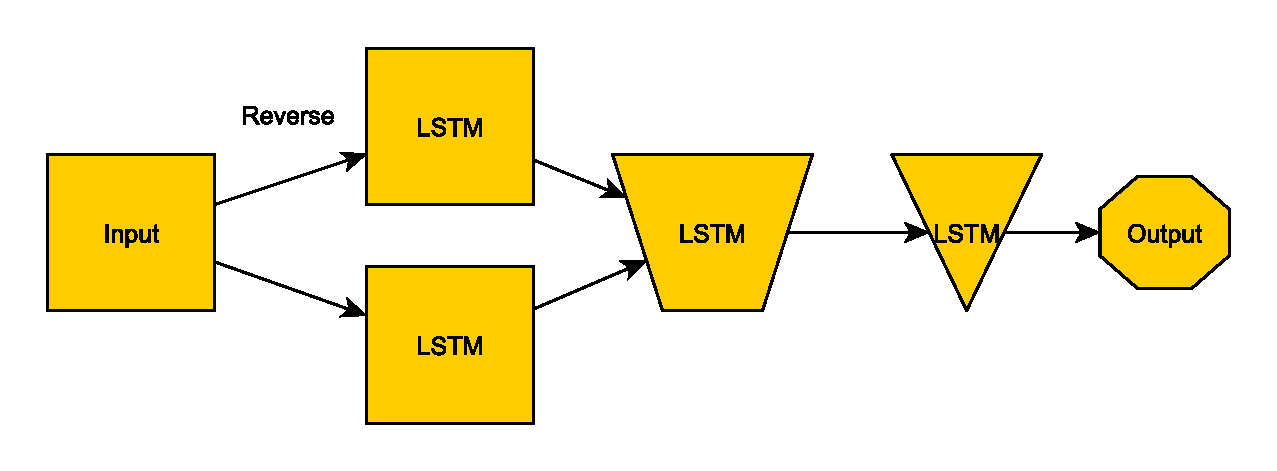
\includegraphics[width=0.7\linewidth]{figures/BiLSTM}
	\caption[modified BiLSTM overview]{Simple diagram of the structure of the BiLSTM. The data from the input layer gets duplicated and passed to two LSTM's where one of them get the data in reverse. When both models have trained on the data they gets concatenated and passed to another LSTM that has half of the units as output. The final LSTM has a single cell as output leaving a single value as the prediction.}
	\label{fig:bilstm}
\end{figure}\todo{Complete caption, and improve figure}

Soil temperatures depend on earlier timestamps, so to make accurate predictions, it's essential to include temperature data from $t, t-1, \dots, t-k$. Evaluating the data both forwards and backwards helps identify features that are noticeable in specific directions. The BiLSTM model, implemented using TensorFlow's Keras module, consists of three layers:\todo{EXPAND}

\begin{itemize}
	\item A Bidirectional LSTM layer for feature extraction.
	\item A regular LSTM layer to condense information with a tanh activation function
	\item An LSTM layer for prediction with a tanh activation function
\end{itemize}

The activation functions used are hyperbolic tangent and sigmoid. The output layer employs the identity function ($f(x) = x$). The hidden layer has half as many recurrent cells as the input layer, and the output layer condenses the hidden layer's output to a single value. For more details, refer to Figure \ref{fig:bilstm} and Table \ref{tab:subtab:BiLSTM_params}.

\begin{table}
	\centering
	\begin{subtable}[t]{0.45\textwidth}
		\begin{tabular}{l|c}
			Parameter name & Range \\\hline\hline
			Epochs & [4,8] \\
			Units & \(\{2^6,2^7,2^8\}\) \\
			Lag time & \(12i\) for \(i \in [1,14]\)
		\end{tabular}
		\caption[Parameter space for modified BiLSTM]{The search space for the modified BiLSTM model. The units define the number of LSTM cells used in the LSTM output. The lag time specifies how many hours the model will take into account when predicting soil temperature. The square brackets indicate an interval including endpoints, while the curly brackets indicate a list of elements.}
		\label{tab:subtab:BiLSTM_params}
	\end{subtable}
	\hfill
	\begin{subtable}[t]{0.45\textwidth}
		\begin{tabular}{l|c}
			Parameter name & Range \\\hline\hline
			Sine terms & [1,10] \\
			Cosine terms & [1,10] \\
			Lag time & [1,14]
		\end{tabular}
		\caption[Parameter space for Plauborg]{The search space for the Plauborg model. The square brackets indicate an interval including endpoints. The "Lag time" indicated the number of time-steps before current time-steps do the model include ($t_{-1},t_{-2},\dots$)}
		\label{tab:subtab:plauborg_params}
	\end{subtable}
	\begin{subtable}[t]{0.45\textwidth}
		\begin{tabular}{l|c}
			Parameter name & Range \\\hline\hline
			Epochs & [4,10]\\
			Lead time & $\{24*n|n\in[1,7]\}$\\
		\end{tabular}
		\caption[Parameter space for BiLSTM and LSTM]{Parameter space for both LSTM and BiLSTM. The square brackets indicate an interval including endpoints. The "Lag time" indicated the number of time-steps before current time-steps do the model include ($t_{-1},t_{-2},\dots$)}
	\end{subtable}
	\caption{Parameter search space for the different deep learning models}
	\label{tab:model_params}
\end{table}

This model is an extention of \citetitle{li_modeling_2020}\cite{li_modeling_2020} written by \citeauthor{li_modeling_2020}. 

\subsubsection{GRU}

The \acrfull{ac:gru} is a simplification of the LSTM cell with fewer total gates, and no output gate. This makes it quicker to train and better for memory deficient computers/servers. The model used in this study is the Keras defult GRU layer. 

GRU shares similarities with \acrshort{ac:lstm} networks but simplifies the architecture by using two gates: the update gate and the reset gate. These gates allow GRU to selectively retain relevant information from previous time steps while avoiding unnecessary washing of information. The update gate determines how much past information should be passed to the future, while the reset gate controls how much past information to forget. GRU has been effective in various sequence modelling tasks.

 \todo{EXPAND, and add formulas}

\subsection{Metrics}\label{sec:method:metric}

The metrics used in this study are

\begin{itemize*}
	\item \acrfull{ac:rmse}
	\item \acrfull{ac:mae}
	\item \acrfull{ac:r2}
	\item bias
	\item \acrfull{ac:kappa}
	\item digit sensitivity
\end{itemize*}

Soil temperatur as a different behaviour than air temperature since energy (temperature) though the soil gets dampen and delayed. Since the data used in this study has outliers that was not cought during data treatment, which has been addresed, the author of this study desided to include two more metrics that are not usually included in the evaluation; The log condition number, and digit sensitivity. Both metrics are based on the calculation of the condition number defined as 

\begin{equation}\label{eq:kappa}
\kappa = \lim\limits_{\varepsilon \to 0^+} \sup\limits_{|\partial x|\leq\varepsilon}  \frac{\left|f(x+\partial x) - f(x)\right|}{|f(x)|}*\frac{|x|}{|\partial x|} 
\end{equation}

Calculating this directly is impossible due to the limitations of handling infinitesimally small numbers in simulations. However, this paper uses a specific algorithm (referred to as $\kappa$) to estimate this value for all the models.

\begin{algorithm}[H]
	\SetAlgoLined
	\KwData{ Data }
	\KwResult{log($\kappa$)}
	Let $\kappa_f$ be the function \ref{eq:kappa}\;
	$\kappa\gets 0$\;
	\For{$i \in {1 \dots |Data|}$}{
		$\partial x \gets \mathcal{U}_{[-\sqrt{\varepsilon/|Data|},\sqrt{\varepsilon/|Data|}]}$\;
		$k \gets$ calculate with $\kappa_f$ from $x$ and $x+\partial x$\;
		\If{k > $\kappa$}{$\kappa \gets k$\;}
	}
	\Return{$\kappa$}
	\caption[Randommised $\kappa$ algorithm]{Method for calculating $\kappa$. $\mathcal{U}$ is a uniform random distrebution in a range.}
	\label{alg:cond_num}
\end{algorithm}

The digit sensitivity is included to give an intuitive understanding of $\kappa$ and is computed simply as $\log_e(\kappa)+1$. This number tells us the significant digit generated from the model. If the number is less than 0 then its the ith digit after the decimal point.

For the rest of the metrics, they are defined as follows
\begin{itemize}
	\item \gls{ac:rmse} = $\sqrt{\frac{\sum (y_{\text{pred}} - y_{\text{truth}})^2}{n}}$
	\item \gls{ac:mae} = $\frac{\sum \left| y_{\text{pred}} - y_{\text{truth}}\right|}{n}$
	\item bias = $\frac{\sum ( y_{\text{pred}} - y_{\text{truth}})}{n}$
	\item \gls{ac:r2} = $1-\frac{\sum (y_{\text{pred}} - y_{\text{truth}})^2}{\sum (y_{\text{pred}} - \vec{y})^2}$
\end{itemize}

Where $\vec{y}$ is the mean of the target, $y_{\text{pred}}$ is the predicted data, and $y_{\text{truth}}$ is the observed soil temperature.

\subsubsection{Model training}

The models get trained on air temperature, however the precise input for each model is not the same for all. The features used for each model are described in table \ref{tab:model_params} and their transformation in table \ref{tab:model_trans}.

The models get a sample of the training data at the time due to the size and the amount for missing data (for example figure \ref{fig:plot-17}) The algorithm used to fetch reliable indexes are demonstrated at algorithm \ref{alg:find_non_nan_ranges_abstract}.

\begin{algorithm}
	\caption{Find Non-NULL Ranges (Abstract)}
	\label{alg:find_non_nan_ranges_abstract}
	\SetKwFunction{FindNonNaNRanges}{FindNonNaNRanges}
	\SetKwInOut{Input}{Input}
	\SetKwInOut{Output}{Output}
	
	\Input{Input data $\text{data}$}
	\Output{List of tuples: $\text{ranges}$}
	
	\BlankLine
	\SetKwData{StartIdx}{start}
	\SetKwData{NonNaNRanges}{ranges}
	\SetKwData{Item}{item}
	
	\FindNonNaNRanges{$\text{data}$}{
		$\NonNaNRanges \gets$ empty list\;
		$\StartIdx \gets$ None\;
		
		\For{$\Item \text{ in } \text{data}$}{
			\If{$\Item is not NULL$}{
				\If{$\StartIdx \text{ is None}$}{
					$\StartIdx \gets \Item$\;
				}
			}
			\Else{
				\If{$\StartIdx \text{ is not None}$}{
					Add ($\StartIdx$, $\Item$ index - 1) to $\NonNaNRanges$\;
					$\StartIdx \gets$ None\;
				}
			}
		}
		\If{$\StartIdx \text{ is not None}$}{
			Add ($\StartIdx$, Last index) to $\NonNaNRanges$\;
		}
		\Return $\NonNaNRanges$\;
	}
\end{algorithm}


\begin{table}[H]
	\centering
	\begin{tabular}{|r|c| p{6cm}|}
		\hline model name & features & transformations \\\hline\hline
		Linear regression & TM & Time get translated to hours by taking the day since new year and multiplying by 24 for then add the hour part. \\\hline
		Plauborg & Time, TM & Time get translated in two way; the current day since new year if looking at daily values, and hours since new year if looking at hourly predictions. When converting TM to daily values the hourly data get averaged. \\\hline
		BiLSTM &Time, TM& Time get translated to hours since new year.\\\hline
	\end{tabular}
	\caption[Model parameters]{Parameters used for predicting soil temperatures at depth 10cm and 20cm.}
	\label{tab:model_trans}
\end{table}

\subsection[Use of AI]{Use of Artificial Intelligence in this paper}

In this paper there has been used Artificial Intelligence (AI), specifically Bing Chat / Copilot hosted by Microsoft Cooperation according to the current guidelines for use of artificial intelligence at the faculty of \acrfull{ac:nmbu}, for the following purposes:

\begin{enumerate}
	\item Formalising sentences and rephrasing sentences.
	\item Spellchecking
	\item Code generation of basic consepts and structures (tree traversal, template for generic classes) 
\end{enumerate}

It is important to emphasize that my engagement with AI have been actively curated and verified with known sources. All code underwent rigorous manual inspection within a dedicated testing environment. Furthermore, no confidential or sensitive information was shared with the AI; my interactions focused solely on broad topics and general inquiries. To validate the accuracy of AI-generated responses, I cross-checked them with established research papers and textbooks.
